\documentclass[11pt, oneside]{article}   	% use "amsart" instead of "article" for AMSLaTeX format
\usepackage[margin = 1in]{geometry}                		% See geometry.pdf to learn the layout options. There are lots.
\geometry{letterpaper}                   		% ... or a4paper or a5paper or ... 
%\geometry{landscape}                		% Activate for rotated page geometry
\usepackage[parfill]{parskip}    		% Activate to begin paragraphs with an empty line rather than an indent
\usepackage{graphicx}				% Use pdf, png, jpg, or eps§ with pdflatex; use eps in DVI mode
								% TeX will automatically convert eps --> pdf in pdflatex		
\usepackage{amssymb, enumerate, tikz, multicol}

%SetFonts

%SetFonts


\title{Math F113X: Homework Set 5}
%\author{The Author}
\date{}							% Activate to display a given date or no date

\begin{document}
\maketitle
%\section{}
%\subsection{}

%Homework assignment 1 is:
%\vspace{-1.5cm}


\fbox{\parbox{\textwidth}{

\begin{itemize}
\item Start with the \emph{introductory problems}, Problems A and B (below)
\item Then, complete the problems from the Graph Theory  section:
\begin{quote}\# 2, 3, 4, 9, 10, 26, 33ab, 34a \end{quote}

\item Answer the following {\bf reflection question}: What did you learn from checking your homework answers against the provided solutions?
\end{itemize}
}}
\begin{multicols}{2}
\textbf{Problem A:} Use the drawing of Graph A (in box) to answer the questions. \\
\fbox{
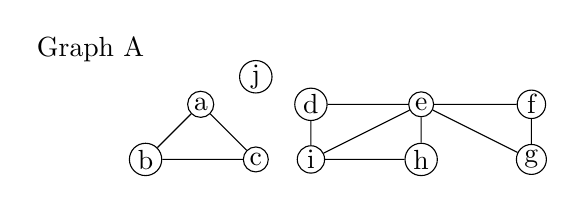
\begin{tikzpicture}[scale=.7]
\node at (-1,2){Graph A};
\node[draw,circle, inner sep=1pt](a) at (1,1){a};
\node[draw,circle, inner sep=1pt](b) at (0,0){b};
\node[draw,circle, inner sep=1pt](c) at (2,0){c};
\draw (a) -- (b) -- (c) -- (a);
\node[draw,circle, inner sep=1pt](d) at (3,1){d};
\node[draw,circle, inner sep=1pt](e) at (5,1){e};
\node[draw,circle, inner sep=1pt](f) at (7,1){f};
\node[draw,circle, inner sep=1pt](g) at (7,0){g};
\node[draw,circle, inner sep=1pt](h) at (5,0){h};
\node[draw,circle, inner sep=1pt](i) at (3,0){i};
\node[draw,circle, inner sep=1pt](j) at (2,1.5){j};
\draw (h) -- (e) -- (d) -- (i)-- (h) -- (e) -- (f) -- (g)-- (e)--(i);
\end{tikzpicture}
}
\begin{enumerate}
\item How many vertices does Graph A have?
\item How many edges does Graph A have?
\item What is the degree of vertex a? Vertex e? Vertex j?
\item For each sequence of vertices, determine if it is a \textbf{path}, a \textbf{circuit}, or \textbf{neither}.
	\begin{enumerate}
	\item $abc$
	\item $abca$
	\item $acid$
	\item $id$
	\item $gfedie$
	\item $gedh$
	\item $a$
	\end{enumerate}
\item Is Graph A connected? Justify your conclusion.
\end{enumerate}

\end{multicols}

\textbf{Problem B:} Which of the graphs below are \textbf{connected}? Which contain \textbf{circuits}? Determine the vertices of \textbf{highest} degree and those of \textbf{lowest} degree.\\
\begin{multicols}{3}
Graph $B_1$\\
\fbox{
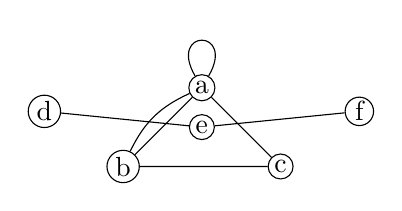
\begin{tikzpicture}
\node[draw,circle, inner sep=1pt](a) at (1,1){a};
\node[draw,circle, inner sep=1pt](b) at (0,0){b};
\node[draw,circle, inner sep=1pt](c) at (2,0){c};
\draw (a) -- (b) -- (c) -- (a);
\node[draw,circle, inner sep=1pt](d) at (-1,0.7){d};
\node[draw,circle, inner sep=1pt](e) at (1,0.5){e};
\node[draw,circle, inner sep=1pt](f) at (3,0.7){f};
\draw (d)--(e)--(f);
\draw[bend right =20] (a) edge (b);
\draw(a) to [out=60, in =120, distance=.7cm] (a);
\end{tikzpicture}
}

\columnbreak
Graph $B_2$\\
\fbox{
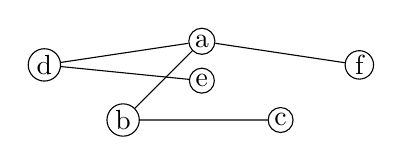
\begin{tikzpicture}
\node[draw,circle, inner sep=1pt](a) at (1,1){a};
\node[draw,circle, inner sep=1pt](b) at (0,0){b};
\node[draw,circle, inner sep=1pt](c) at (2,0){c};
\draw (a) -- (b) -- (c);
\node[draw,circle, inner sep=1pt](d) at (-1,0.7){d};
\node[draw,circle, inner sep=1pt](e) at (1,0.5){e};
\node[draw,circle, inner sep=1pt](f) at (3,0.7){f};
\draw (a)--(d)--(e)(a)--(f);
\end{tikzpicture}
}

\columnbreak

Graph $B_3$\\
\fbox{
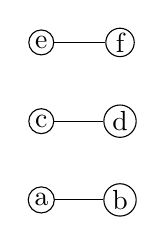
\begin{tikzpicture}
\node[draw,circle, inner sep=1pt](a) at (0,0){a};
\node[draw,circle, inner sep=1pt](b) at (1,0){b};
\node[draw,circle, inner sep=1pt](c) at (0,1){c};
\node[draw,circle, inner sep=1pt](d) at (1,1){d};
\node[draw,circle, inner sep=1pt](e) at (0,2){e};
\node[draw,circle, inner sep=1pt](f) at (1,2){f};
\draw (a)--(b)(c)--(d)(e)--(f);
\end{tikzpicture}
}
\end{multicols}
\hrulefill

Remember to write up your homework solutions according to the homework writeup guidelines. 

Homework is graded using the following rubric for each problem (or problem part):

\begin{description}
\item[2 points:] You provided a complete answer, with supporting work, written up clearly
\item[1 point:] Some attempt at a solution, but incomplete writeup / unclear / illegible / no answer
\item[1 point:] Only an answer, with no supporting work 
\item[0 points:] Missing.
\end{description}

After you do the homework, you need to check your answers against the solutions! Then figure out your errors (if any) and revise your homework before you submit it. Finally, answer the reflection question.

Homework must be submitted on Gradescope.

\end{document}  